\section{Architekturen}
\label{Archs}

In diesem Abschnitt werden die verwendeten Architekturen vorgestellt.

\subsection{Problemstellung}
Alle in dieser Bachelorarbeit verwendeten Architekturen, wurden von ihren Entwicklern für eine Anwendung im Bereich der zweidimensionalen Bildklassifizierung implementiert. Die Eingabedaten liegen in diesem Fall allerdings als vierdimensionaler Tensor mit Abmessung 8x84x84x1 vor. Dadurch mussten in den problemspezifischen Implementationen dieser Arbeit Anpassungen an Filtereinstellungen vorgenommen werden, ohne die grundlegende Struktur der Architekturen zu verändern. In den vorgestellten Modellen wird die Tiefe in den Convolutional Layern ignoriert und jede der 8 Schichten wird einzeln von den Filtern bearbeitet, daher verfügen alle Pooling und Convolutional Filter über Dimension des Schemas [1,X,X], wobei gilt $X \in \mathbb{N}$, $X \geq 1$. Erst in den Fully-Connected Layern werden alle Schichten zusammen betrachtet. 

Da die Architekturen über stark variierende Parameterzahlen verfügen und durch sehr tiefe Strukturen mitunter zu Umfangreich für die vorhandenen Rechenressourcen sind, wurden die Parameter einiger Architekturen angepasst, sodass alle Architekturen einen ähnlichen Umfang -- gemessen an der Parameteranzahl -- haben. Dieser Umstand schafft gleichzeitig eine bessere Vergleichbarkeit der Strukturen aller Architekturen, da Abweichungen durch wesentlich höhere Parameterzahlen ausgeschlossen werden können. 

Viele gängige Implementationen der vorgestellten Architekturen setzen zudem Global Average Pooling vor den Fully-Connected Layern ein. Da in dieser Arbeit jedoch zwei gegeneinander arbeitende Faktoren in einem Bild miteinander verglichen werden, wird die Matrix lediglich auf $2 \times 2$ durch Average-Pooling reduziert. Infolgedessen erhält der Fully-Connected Layer 2 Werte pro Armee mit denen er weiter rechnen kann. 
 
\subsection{Baseline}
Um die Effektivität der Architekturen zu überprüfen wurde eine Baseline implementiert, welche nach einer festen Implementierung die Gefechts-Ausgänge berechnet. Die Baseline berücksichtigt sowohl die Offensive Kampfkraft der beiden Armeen, als auch die defensiven Eigenschaften jeder Armee. 

Die Offensive Kampfkraft der Armeen wird durch einen \textit{Powervalue} dargestellt. Der Powervalue errechnet sich aus dem Angriffswert folgend Damage-per-second (DPS, zu Deutsch: Schaden pro Sekunde) zusammen mit sämtlichen Boni, welche durch die unterschiedlichen Einheitenklassen hinzukommen. So sind manche Einheiten beispielsweise effektiver gegen Einheiten welche dem mechanischen Typ angehören. 

Der Powervalue errechnet sich in etwa wie folgt:
\begin{algorithmic}[1]
\Procedure {PowervalueMitBoni}{$einheit$, $gegner$}
	\State \Comment jeder Bonustyp beinhaltet einen Wert typ, als Identifikator und einen Wert Schaden.
	\State $bonustyp \leftarrow einheit[bonustyp]$
	\State \Comment Für jeden Bonustyp, den die Einheit beinhaltet..
	\ForAll {$bt \in bonustyp$}
		\If {$gegner[bonustyp] = bt[typ]$}
			\State \Comment berechne anteilig den Bonusschaden der aktuellen Einheit
			\State $faktor \leftarrow anzahl(gegner[bt]) \div anzahl(gegner)$
			\State $bonus \leftarrow bonus + bt[schaden] \times faktor$
		\EndIf
	\EndFor
	\State $schaden = einheit[basisschaden] + bonus$
	\State \textbf{return} $schaden$
\EndProcedure
\end{algorithmic}

Da Einheiten immer nur eine bestimmte Art von Einheiten angreifen können, errechnet der Algorithmus insgesamt 4 Werte. Für jedes der beiden Teams wird der Wert für Schaden an Bodeneinheiten und der Wert für Schaden an Lufteinheiten errechnet. Zusätzlich wird ein Powervalue in Relation zur Einheiten Verteilung Luft-Boden errechnet:
\begin{algorithmic}[1]
\State $Boden\_Faktor = anzahl(gegner['Boden']) \div anzahl(gegner)$
\State $Luft\_Faktor = anzahl(gegner['Luft']) \div anzahl(gegner)$
\State $powervalue\_gesamt \leftarrow schaden['Boden'] * Boden\_Faktor + schaden['Luft'] * Luft\_Faktor$ 
\end{algorithmic}



Um die Überlebensfähigkeit der Armeen zu bestimmen werden die Hitpoints der Einheiten sowie deren Schilde herangezogen. Auch hier wird bei beiden Armeen zwischen Luft und Bodeneinheiten unterschieden. Somit wird eine Vergleichbarkeit zwischen dem Durchhaltevermögen eigener Luft- bzw. Bodentruppen und Luft- bzw. Boden-DPS der Gegenseite geschaffen.

\begin{algorithmic}[1]
\Procedure {Überlebensfähigkeit}{einheiten}
	\ForAll {$einheit \in einheiten$}
		\If {$einheit[typ] = "Boden"$}
			\State $abwehr[Boden] \leftarrow abwehr[Boden] + einheit[leben] + einheit[schild]$
		\EndIf
		\If {$einheit[typ] = "Luft"$}
			\State $abwehr[Luft] \leftarrow abwehr[Luft] + einheit[leben] + einheit[schild]$
		\EndIf
	\EndFor 
	\State \textbf{return} $abwehr[Boden], abwehr[Luft]$
\EndProcedure
\end{algorithmic}

Die beiden letzten Charakteristika bzgl. beider Armeen sind Aufklärung und Unsichtbarkeit. Sie werden durch boolsche Werte ausgedrückt, welche dann Wahr sind wenn mindestens eine Einheit in der Armee über die entsprechende Fähigkeit verfügt. Die Werte fließen in den Wert \textit{fightable} mit ein, welcher bestimmt, ob eine Armee überhaupt in der Lage ist alle Einheiten der anderen Seite zu attackieren. Fightable ist dann Wahr, wenn die Armee alle in der Gegnerarmee enthaltenen Einheitentypen (Luft/Boden) angreifen kann. Sollte der Gegner über Unsichtbare Einheiten verfügen, so ist fightable genau dann Wahr, wenn die Armee über Einheiten verfügt, die aufklären können.

Als Entscheider-Funktion wurden zunächst lediglich die beiden Team\_Werte aus der Prozedur \textbf{Entscheider} Zeile 19 folgend verglichen. In Tabelle \ref{classficationohneremis} wird der aus den berechneten Labeln und mit Scikit-Learn erstellte Classification-Report veranschaulicht. Es ist sowohl eine F1-Score von 0.67 abzulesen. Der Nachteil der Methode ist, dass Remis als Ausgang nicht in Betracht gezogen werden.  

\begin{table}
\centering
\caption{Classification-Report ohne Remis}
\begin{tabular}{@{}lllll@{}}
\hline
& precision & recall & f1-score & support\\
Minerals & 0.71 & 0.74 & 0.72 & 56027\\
Vespene & 0.61 & 0.58 & 0.59 & 39921\\
 avg / total & 0.67 & 0.67 & 0.67 & 95948\\
\hline
\end{tabular}
\label{tb:classificationohneremis}
\end{table}

Um Remis zu evaluieren müssen zunächst die Gründe für ein Remis erörtert werden. Als naive Grundlage wird zunächst die Annahme herangezogen, dass ein Remis dann auftritt, wenn beide Armeen sich nicht attackieren können. Die Prozedur \textbf{Entscheider} wird und den Zeilen 2-3 modifiziert, indem die Fightable-Variablen beider Teams abgefragt werden. Für den Fall dass beide Seiten ein Falsch zurückgeben, gibt der Entscheider eine 2 für Remis zurück. Tabelle \ref{tb:classificationmitremisnaiv} zeigt den Classification-Report dieses Ansatzes.  precision, recall und f1-score sind für die Siege beider Seiten stark gesunken und die Genauigkeit der Auswertung liegt bei etwa 47,91\%.  

\begin{table}
\centering
\caption{Classification-Report mit naiver Remis-Evaluation}
\begin{tabular}{@{}lllll@{}}
\hline
& precision & recall & f1-score & support\\
Minerals & 0.66 & 0.43 & 0.52 & 56027\\
Vespene & 0.47 & 0.54 & 0.50 & 39921\\
Remis & 0.32 & 0.50 & 0.39 & 25032\\
 avg / total & 0.53 & 0.48 & 0.49 & 120980\\
\hline
\end{tabular}
\label{tb:classificationmitremisnaiv}
\end{table}

Bei genauer Beobachtung der Gefechte fällt in der Folge auf, dass Gefechte nicht nur Unentschieden ausgehen, wenn beide Teams nicht angreifen können, sondern auch wenn beide Teams sich durch töten einiger Einheiten eines bestimmten Typs in ein Remis kämpfen. Ein weiterer Fall für ein Remis ist durch die zeitliche Einschränkung der Replay-Generierung gegeben. Sollte ein Team nur über wenige Einheiten eines bestimmten Typs verfügen, so kann es sein, dass diese Einheiten fightable zu Wahr evaluieren lassen. Da es aber zu wenige Einheiten sind, schaffen sie es nicht die relevanten Gegnereinheiten in der vorgegebenen Zeit zu töten und der Generator bricht das Gefecht mit einem Remis als Ergebnis ab. Daher wird der Entscheider um die Zeilen 5 bis 17 erweitert. Hier wird die Fähigkeit bestimmt eine Armee in gegebener Zeit zu vernichten. Die Gleichung tritt in Kraft, sobald eine Armee -- durch die Zusammensetzung der beiden Armeen -- nicht komplett zerstört werden kann. In diesem Fall bestimmt der Algorithmus, ob diese Armee im Rahmen der zeitlichen Vorgaben den Sieg erringen kann, sprich genug Schaden verursachen kann um die andere Armee zeitnah zu zerstören. Die Konstante in der Berechnung der Schadenswerte in der Zeilen 6 und 13 wurde durch empirisch durch Ausprobieren ermittelt. Abbildung \ref{fig:konstante_baseline} zeigt den F1-Score und die Genauigkeit unter Berücksichtigung verschiedener Werte für die Konstante. Das Maximum wird beider Werte liegt bei ca. 21. Der Classification-Report für Konstante=21 ist in Tabelle \ref{tb:classificationcomplete} dargestellt. Die Genauigkeit für diese Variante liegt bei ca. 51\% und bringt somit einen Zugewinn von 3,09 Prozentpunkten.

\begin{table}
\centering
\caption{Classification-Report mit kompletter Remis-Evaluation}
\begin{tabular}{@{}lllll@{}}
\hline
& precision & recall & f1-score & support\\
Minerals & 0.70 & 0.48 & 0.57 & 56027\\
Vespene & 0.54 & 0.51 & 0.53 & 39921\\
Remis & 0.32 & 0.58 & 0.41 & 25032\\
 avg / total & 0.57 & 0.51 & 0.52 & 120980\\
\hline
\end{tabular}
\label{tb:classificationcomplete}
\end{table}

\begin{algorithmic}[1]
\Procedure {Entscheider}{schaden, abwehr, fightable}
\If {$\neg fightable['A'] \land \neg fightable['B']$}
	\State \textbf{return} 2 \Comment Beide Armeen können sich nicht angreifen -> Remis
\EndIf
\If {$fightable['A']  \land \neg fightable['B']$}
	\If {$schaden['A'][Boden] * 21 \geq abwehr['B'][Boden] \land schaden['A'][Luft] * 21 \geq abwehr['B'][Luft]$}
		\State \textbf{return} 0 \Comment Team A siegt
	\Else 
		\State \textbf{return} 2 \Comment Team A schafft Sieg nicht innerhalb der Zeit
	\EndIf
\EndIf
\If {$\neg fightable['A'] \land fightable['B']$}
\If {$schaden['B'][Boden] * 21 \geq abwehr['A'][Boden] \land schaden['B'][Luft] * 21 \geq abwehr['A'][Luft]$}
	\State \textbf{return} 1 \Comment Team B siegt
\Else 
	\State \textbf{return} 2 \Comment Team B schafft Sieg nicht innerhalb der Zeit
\EndIf
\EndIf
\State $team\_wert\_A \leftarrow schaden['A'][Gesamt] + abwehr['A'][Boden] + abwehr['A'][Luft]$
\State $team\_wert\_B \leftarrow schaden['B'][Gesamt] + abwehr['B'][Boden] + abwehr['A'][Luft]$

\If {$team\_wert\_A > team\_wert\_B$}
	\State \textbf{return} 0 \Comment Team A besiegt Team B
\Else
	\State \textbf{return} 1 \Comment Team B besiegt Team A
\EndIf
\EndProcedure
\end{algorithmic}


\begin{figure}[H]
\centering
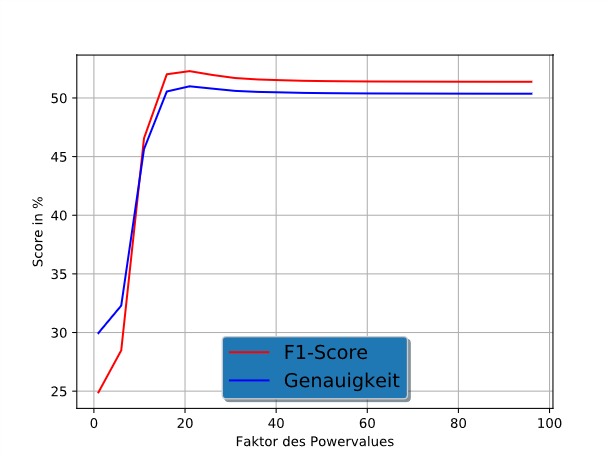
\includegraphics[scale=0.8]{pictures/konstantenVollesModell}
\label{fig:konstante_baseline}
\end{figure}
 
\subsection{All-Convolutional Net}
Das All-Convolutional Net von Springenberg et al. \parencite{DBLP:journals/corr/SpringenbergDBR14} ist eine CNN-Architektur, die g\"anzlich auf den Gebrauch von Max-Pooling Layern verzichtet. Die Reduzierung der Dimensionen wird durch den Einsatz von \textit{Convolutional Layern} mit einem entsprechenden stride-Parameter vollzogen. In Experimenten basierend auf dem CIFAR-10 Datensatz erreichten die vorgestellten Architekturen eine Fehlerrate von weniger als 10\% und zeigten im Vergleich zu Modellen mit Max-Pooling äquivalente oder sogar bessere Fehlerraten. Tabelle \ref{tb:arch_allcnn} zeigt die Parameterzahlen der in dieser Bachelorarbeit genutzten Architektur, welche in Abbildung \ref{fig:arch_allcnn} dargestellt ist. Die Tabelle listet in der Layer-Spalte zuerst die Filtergr\"o\ss{}e, dann die Filteranzahl und nachfolgend gegebenenfalls den stride- und den padding-Parameter mit auf. Sollten diese nicht aufgef\"uhrt sein, gilt \textit{stride=(1,1,1)} und \textit{padding='same'}. Die Ausgabedimension ist im Format \textit{channels last} (zu Deutsch: \textit{Kanäle zuletzt}) angegeben. 

\begin{table}
\centering
\caption{All Convolutional Neural Network - Architektur}
\begin{tabular}{@{}lll@{}}
\hline
Layer & Ausgabedimension & Parameter\\
\hline
Eingabe & 8 x 84 x 84 x 1 & \\
3x3 Conv, 96 & 8 x 84 x 84 x 96 & 960\\
3x3 Conv, 96 & 8 x 84 x 84 x 96 & 83.232\\ 
3x3 Conv, 96/s=2 V & 8 x 41 x 41 x 96 & 83.232\\ 
3x3 Conv, 192 & 8 x 41 x 41 x 192 & 166.464\\
3x3 Conv, 192 & 8 x 41 x 41 x 192 & 332.352\\
3x3 Conv, 192/s=2 V & 8 x 20 x 20 x 192 & 332.352\\
3x3 Conv, 192 & 8 x 20 x 20 x 192 & 332.352\\
1x1 Conv, 192 & 8 x 20 x 20 x 192 & 37.440\\
1x1 Conv, 10 & 8 x 20 x 20 x 10 & 1.950\\
10x10 Average Pooling & 8 x 2 x 2 x 10 & \\
Output Layer (FCL), Units=3 & & 963\\
\hline
Summe Variablen & & 1.371.297\\
\hline
\end{tabular}
\label{tb:arch_allcnn}
\end{table}

\begin{figure}[H]
\centering
\caption{Architektur des All-Convolutional CNN}
\includegraphics[angle=90, scale=0.5]{pictures/inception/AllConvCNN}
\label{fig:arch_allcnn}
\end{figure}

\subsection{ResNet}
\label{sek:resnet}
ResNet ist eine von \textcite{He_2016} vorgestellte Architektur, welche sich Shortcut Connections (zu deutsch etwa: \textit{abkürzende Verbindungen}) zu nutze macht. Mit zunehmender Tiefe von CNNs wurde bei einigen Problemstellungen festgestellt, dass tiefere CNNs an Genauigkeit verlieren können, was im Allgemeinen der intuitiven Einschätzung widersprach, da man sich von dem Einsatz zusätzlicher Layer eine steigende Präzision erwartete. Da eine Evaluierung der Gradienten des entsprechenden CNNs das Vanishing Gradient Problem (zu deutsch etwa: \textit{verschwindende Gradienten Problem}) ausschloss, wurde die Vermutung aufgestellt, dass die Layer im CNN leichter sogenannte \textit{zero mappings} ($f(x) = 0$) lernen und daher nicht die Identitätsfunktion ($f(x) = x$). Als mögliche Lösung werden im Deep Resiual Neural Network shortcut connections eingefügt, welche ausschließlich als Identitätsfunktion dienen. 

Abbildung \ref{fig:resnet} zeigt die Implementation eines ResNets mit acht Residual Blöcken. Die Eingabe wird zunächst von einem Convolutional Layer mit 7x7 Filtergröße und Stride=2 verarbeitet um die Dimensionen der Eingabe zu reduzieren. Nachfolgend werden diverse Residual Blöcke hintereinander gereiht. Die Residual Blöcke bestehen aus zwei Convolutional Layern mit einer Filtergröße von 3x3 und werden von einer Residual Connection überbrückt. Diese bildet in allen Blöcken mit Ausnahme von Block 6 die Identität der Eingabematrizen ab und wird nach den beiden Convolutional Layern hinzu addiert. Da Block 6 die Dimensionen in Höhe und Breite der Eingabe durch einen Stride-Parameter=2 reduziert und zugleich die Anzahl der Kanaldimensionen auf 128 erhöht, muss die Residual Connection mittels eines Convolutional Layers die gleichen Berechnungen vollziehen. Daher besteht in diesem Fall die Residual Connection aus einem Convolutional Layer mit Filtergröße 3x3 und Stride=2. Nach den Residual Blöcken werden die Daten wie bei Inception V4 mittels Average Pooling auf die Dimensionen 8x2x2x128 (Kanalanzahl) reduziert und danach von einem FCL mit 64 Einheiten weiterverarbeitet. Der Ausgabelayer wird von einem FCL mit drei Einheiten gebildet. Tabelle \ref{tb:resnet} listet die Anzahl der Parameter auf.
\newpage
\begin{figure}[H]
\thispagestyle{empty}
\centering
\caption[Caption for LOF]{ResNet mit acht Residual Blöcken}
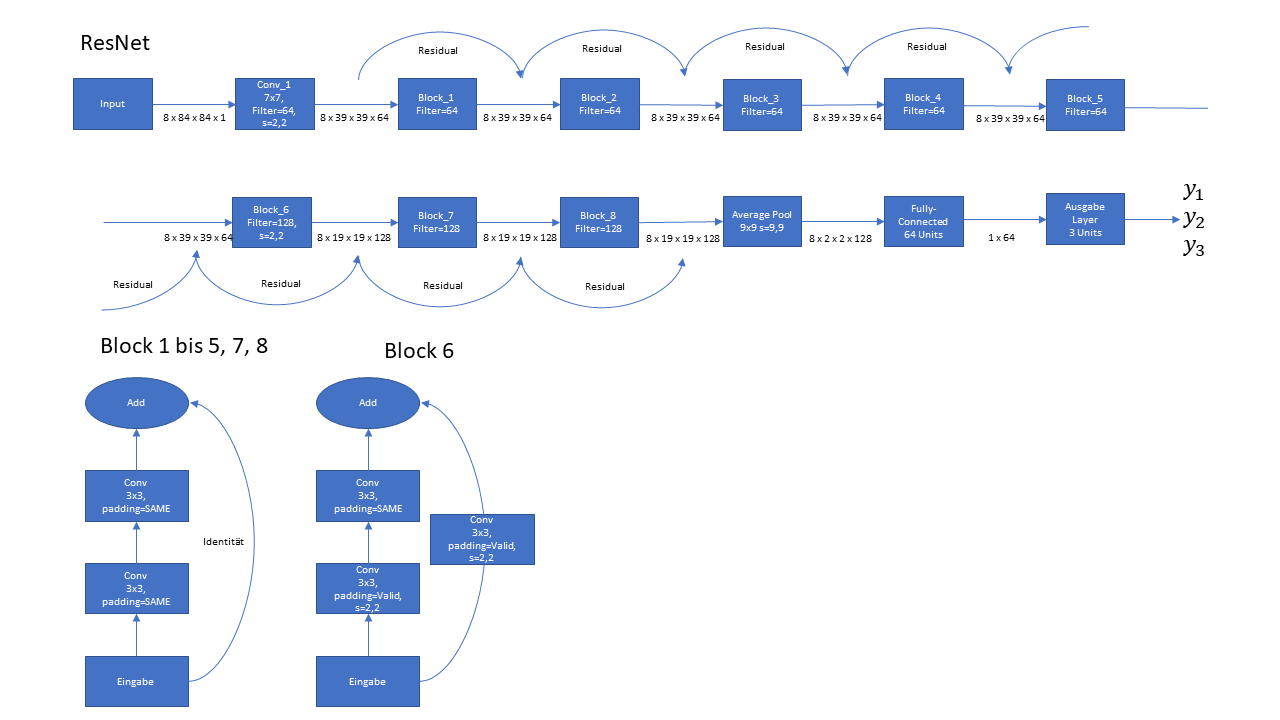
\includegraphics[angle=90, scale=0.65]{pictures/Inception/ResNet}
\label{fig:resnet}
\end{figure}

\begin{table}
\centering
\caption{ResNet: Auflistung der Variablenzahl.}
\begin{tabular}{@{}lr@{}}
\hline
Block & Parameter\\
\hline
7x7 Conv &  3.328\\
Block 1 & 73.984\\
Block 2 & 73.984\\
Block 3 & 73.984\\
Block 4 & 73.984\\
Block 5 & 73.984\\
Block 6 & 295.552\\
Block 7 & 295.424\\
Block 8 & 295.680\\
FCL Units=64 & 262.208\\
Ausgabe Layer & 195\\
\hline
Summe Variablen & 1.522.307\\
\hline
\end{tabular}
\label{tb:resnet}
\end{table}

\subsection{Inception V4}
\label{sek:incv4}
Inception V4 ist eine CNN-Architektur vorgestellt von \textcite{DBLP:journals/corr/SzegedyIV16}. Sie f\"uhrt drei verschiedene Module, sowie zwei Reduction-Bl\"ocke als Bausteine des Netzes ein. Die Zusammensetzung der Bausteine ist in den folgenden Abbildungen \ref{fig:incv4}, \ref{fig:stem}, \ref{fig:incmod} und \ref{fig:incred} dargestellt.

Im Vergleich zu früheren Versionen der Inception-Architekturen konnte die Trainingsgeschwindigkeit durch das Nutzen von Residual Connections drastisch erhöht werden. Zudem erreichten die neuen Versionen der Architektur verglichen mit Inception-v3 und ResNet-151 bessere Leistungen in Tests auf dem ILSVRC 2012 Datensatz \parencite{DBLP:journals/corr/SzegedyIV16}.

\begin{figure}[H]
\centering
\caption[Caption for LOF]{Übersicht der Inception V4-Architektur}
\includegraphics[angle=90, scale=0.8]{pictures/inception/InceptionV4}
\label{fig:incv4}
\end{figure}

Abbildung \ref{fig:incv4} zeigt den allgemeinen Aufbau der Inception V4 Netzwerkes. Filter sind mit der Filtergröße und Filteranzahl, sowie gegebenenfalls Stride (s) und Padding (Vaild) aufgeführt. Sofern Stride und Padding fehlen, gilt Stride=1 und Padding=\textit{same}. Die Dimensionen sind an den Pfeilen zwischen den Layern aufgeführt und nach dem Format \textit{channels last} formatiert. Im Vergleich zu der Vorlage von \textcite{DBLP:journals/corr/SzegedyIV16} wurde Filteranzahl eines jeden Layers durch 4 geteilt um die Parameterzahl in dem Bereich der anderen Architekturen zu halten. Zur Normalisierung wird im Allgemeinen Batch Normalization genutzt, welches nach der Konkatenation in jedem Block zur Anwendung kommt. 

Die Eingabe wird zunächst vom STEM-Block verarbeitet, welcher in Abbildung \ref{fig:stem} detailliert erläutert wird. Er dient im Netzwerk als Eingabelayer und dient der ersten Verarbeitung der Daten sowie der Reduktion der Bilddimensionen durch Pooling und entsprechende Padding-Einstellungen. Daraufhin werden die Daten an das erste Inception-Modul (Inception-A Abbildung \ref{fig:incmod}) übergeben. Das Inception-A-Modul wird von einer Residual Connection überbrückt. Das Verfahren ist der ResNet-Architektur aus Sektion \ref{sek:resnet} entlehnt. In dieser Architektur wird die Residual Connection mittels eines 1x1 Convolutional Filters auf die passende Anzahl an Kanälen dimensioniert. Das Inception-A-Modul in Verbindung mit der Residual Connection kann beliebig oft hintereinander gereiht werden, um die gewünschte Tiefe des Netzwerks zu erlangen, da sich die Dimensionen mit fortlaufender Aneinanderreihung nicht verändern. Unter Berücksichtigung der Parameterzahl des Netzwerks, verfügt das Netzwerk jedoch nur über ein Inception-A-Modul, bevor es in das Reduction-A-Modul (Abbildung \ref{fig:incred}) übergeht. Im Reduction-A-Modul werden die Dimensionen der Eingabedaten entlang der zweiten und dritten Achse reduziert während sich die Anzahl der Kanäle von 96 auf 288 erhöht. Er folgen Inception-B (Abbildung \ref{fig:incmod}) und Reduction-B (Abbildung \ref{fig:incred}), welche nach dem selben Muster verfahren. Das Inception-Modul verarbeitet die Daten auf vier verschiedenen Pfaden und übergibt diese an das Reduction-Modul um erneut die Dimensionen der Höhe und Breite auf 8x8 zu reduzieren. Auch das Inception-B-Modul wird von einer Residual Connection überbrückt und kann zusammen mit dieser Verbindung beliebig oft in Reihe geschaltet werden. Den Abschluss der Convolutional Layer bildet das Inception-C-Modul (Abbildung \ref{fig:incmod}). Nachfolgend wird mittels Average Pooling die Eingabe auf 8x2x2x384 reduziert und als Vektor an den FCL übergeben. Die Auswertung zu den drei Klassen findet in dem zweiten FCL statt, welcher lediglich aus drei Einheiten besteht. 

\begin{figure}[H]
\centering
\caption[Caption for LOF]{STEM-Modul}
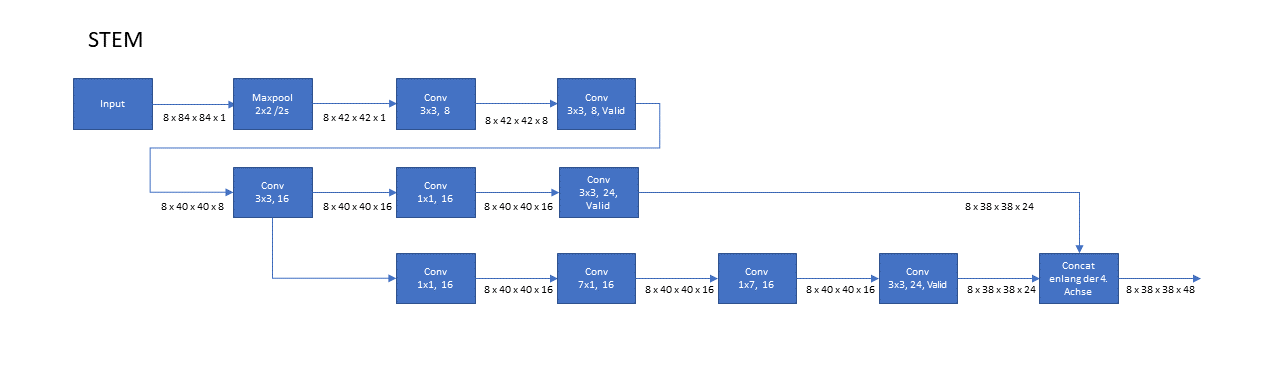
\includegraphics[angle=90, scale=0.65]{pictures/Inception/STEM}
\label{fig:stem}
\end{figure}

Der STEM-Block aus Abbildung \ref{fig:stem} bildet die Eingabeschicht der Architektur, welcher die ersten Berechnungen vollzieht und gleichzeitig der ersten Reduzierung der Bilddimensionen dient. In dieser Version sind nicht alle dimensionsreduzierenden Elemente des STEM-Blocks aus \textcite{DBLP:journals/corr/SzegedyIV16} enthalten, da die Eingabedimension der Daten dieser Arbeit wesentlich geringer ist, als die Bildgröße des ILSVRC 2012 Datensatzes (84x84 im Vergleich zu 299x299), somit ist eine weitere Reduktion der Daten vor Einführung des ersten Inception-Moduls nicht notwendig. Nach anfänglicher Verarbeitung durch einige Convolutional Layer, werden die Daten auf zwei Wegen weiterverarbeitet. Der erste Weg arbeitet mit quadratischen Filtergrößen, während der zweite Weg mit rechteckigen Filtergrößen in Reihe arbeitet. Beide Wege werden vor der Weitergabe an das nächste Modul entlang der Kanalachse (4. Achse) konkateniert, sodass aus den beiden Ausgaben mit Dimensionen 8x38x38x24 eine einzige Ausgabe mit 8x38x38x48 entsteht. Diese wird an das Inception-A-Modul weitergegeben. 

\begin{figure}[H]
\centering
\caption[Caption for LOF]{Übersicht der Inception V4-Module A,B und C}
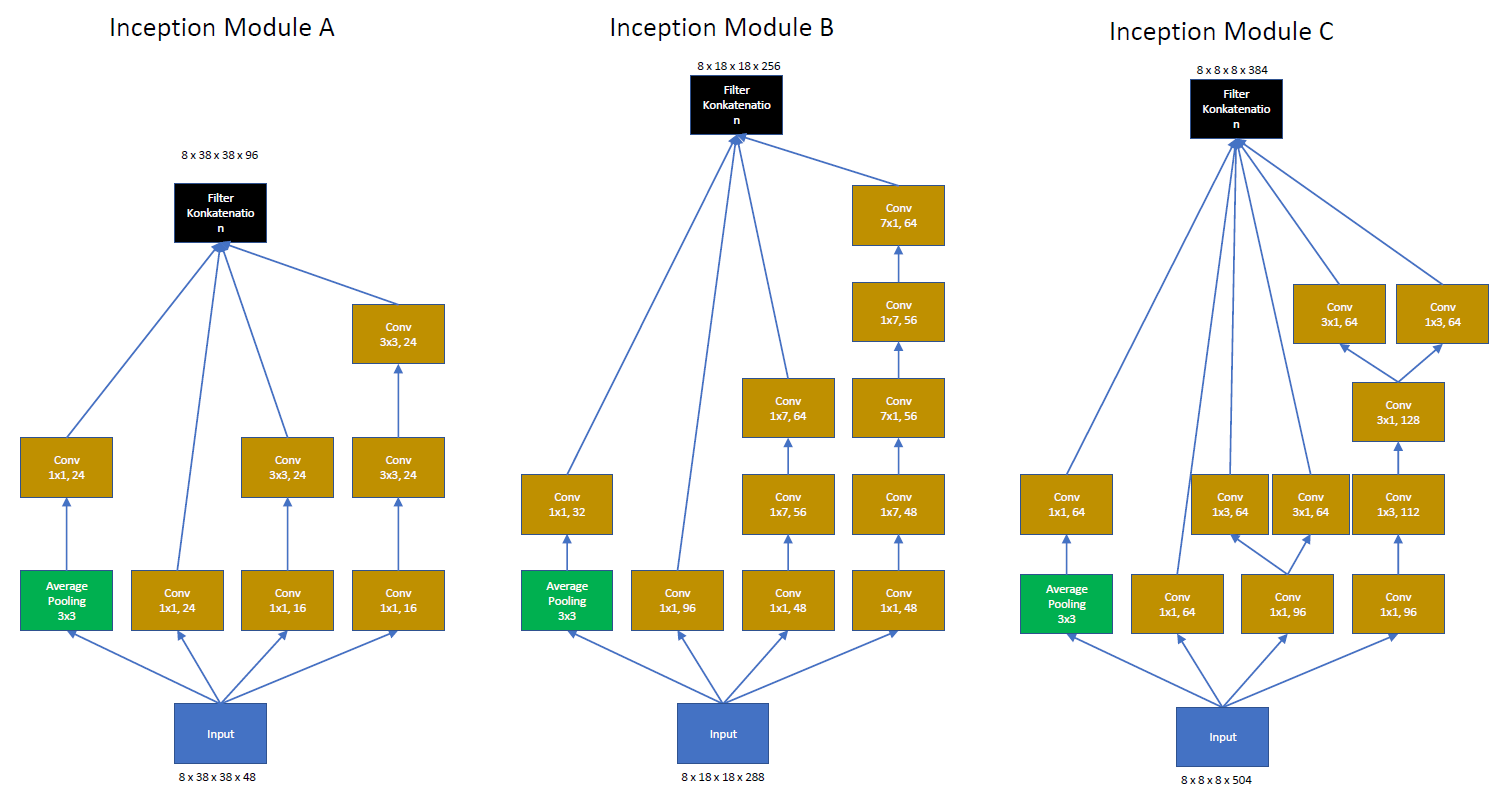
\includegraphics[scale=0.3]{pictures/Inception/InceptionABC}
\label{fig:incmod}
\end{figure}

Die Inception-Module (Abbildung \ref{fig:incmod}) sind speziell für ihre Eingabegrößen angepasst. Alle Module spalten sich aus den Eingabedaten heraus in 4 Wege ab. In Modul C spalten sich zwei Wege erneut auf. Jedes Modul nutzt 1x1 Convolutional Layer um die Dimensionen der Eingabe vor der Verarbeitung oder Weitergabe zu reduzieren. Diese Layer findet man auf den drei rechten Wegen an erster Stelle und auf dem linken Weg nach dem Average Pooling in allen Modulen. Die Unterschiede zwischen den Modulen findet man hauptsächlich auf der rechten Seite aller Module, da sich die Convolutional Layer links lediglich durch die Filteranzahl unterscheiden. Auf der rechten Seite der Module lässt sich erkennen, dass Modul A auf symmetrische Filter setzt. Die Module B und C arbeiten jedoch mit asymmetrischen Filtern, welche meist entgegengesetzt angeordnet sind (3x1 folgt auf 1x3). Die rechten Wege in Modul B sind drei, bzw. fünf Layer tief und mit Filtern der Maße 1x7 und 7x1. In Modul C hingegen spalten sich die Wege nach einem und drei Layern auf und die Filter arbeiten mit 3x1 und 1x3 Layouts. Alle Module konkatenieren schlussendlich ihre vier bzw. sechs Verarbeitungspfade entlang der Kanalachse, bevor die Daten den nächsten Layer erreichen.

\begin{figure}[H]
\centering
\caption[Caption for LOF]{Übersicht der Inception V4-Reduktions-Module A und B}
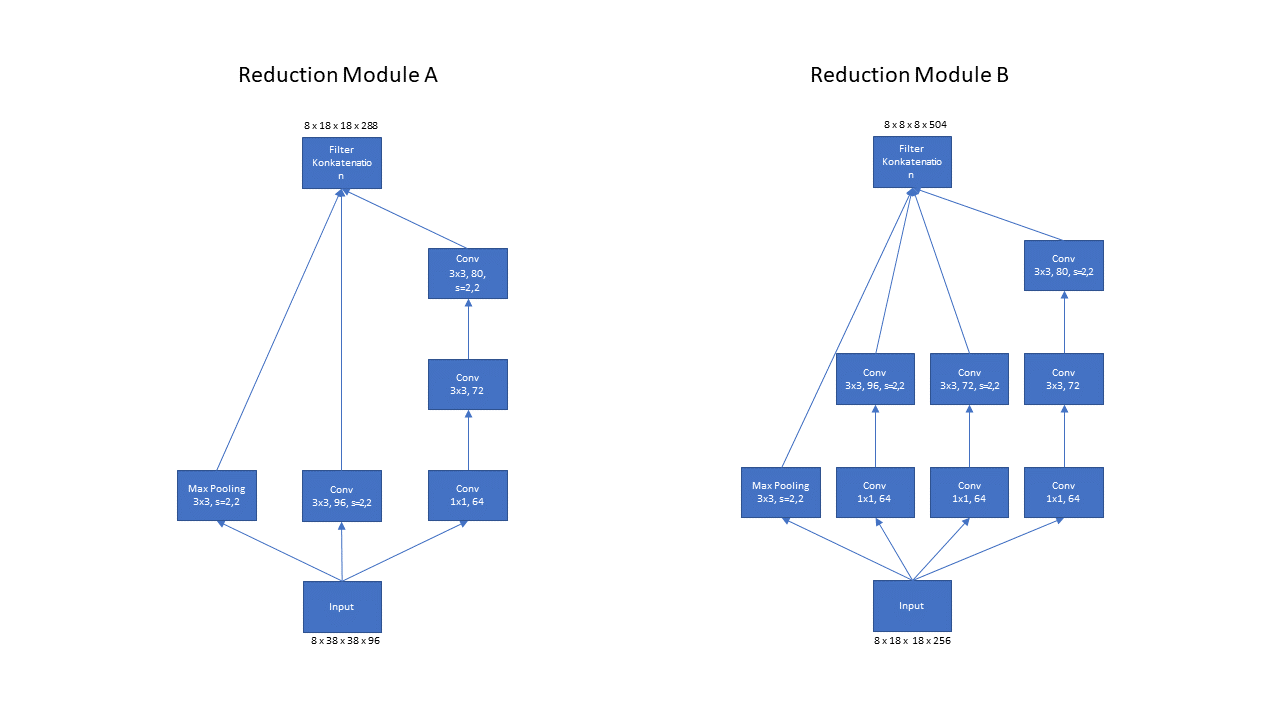
\includegraphics[scale=0.3]{pictures/Inception/Reduction}
\label{fig:incred}
\end{figure}

Zur Reduzierung der Bilddimensionen Höhe und Breite nutzt Inception Reduction-Module (Abbildung \ref{fig:incred}). Beide Module nutzen sowohl Max-Pooling als auch Convolutional Layer mit Stride=2 um die Dimensionen der Eingabedaten entsprechend zu reduzieren. Reduction-A nutzt lediglich auf der rechten Seite des Moduls einen 1x1 Filter um die Dimensionen der Daten zu reduzieren. Bei Reduction-B kommt diese Methode bei den drei rechten Wegen zum Einsatz. In beiden Modulen wird mit 3x3 Filtern gearbeitet. Diese Filter reduzieren die Größe der Eingabedaten bzlg. Höhe $H^i$ und Breite $W^i$ wie folgt: $W^o = W^i / 2 - 1$ und $H^o = H^i / 2 - 1$. $W^o$ und $H^o$ stehen hier entsprechend für die Breite und Höhe der Ausgabe. Auch in den Reduction-Modulen werden die Ergebnisse der einzelnen Berechnungspfade zuletzt entlang der Kanalachse konkateniert. 

Tabelle \ref{tb:var_inc4} zeigt die einzelnen Module der Inception Architektur und ihre Variablenzahlen. In den Zahlen f\"ur Inception A, B und C sind die Variablen der Residual Network Verbindungen mit eingerechnet. 

\begin{table}
\centering
\caption{Inception V4 und V4-SE: Auflistung der Variablenzahl.}
\begin{tabular}{@{}lrr@{}}
\hline
Block & Parameter V4 & Parameter V4-SE\\
\hline
STEM &  13.048 & 13.048\\
Inception A & 20.984 & 21.008\\
Reduction A & 182.144 & 182.144\\
Inception B & 265.464 & 224.568\\
Reduction B & 240.752 & 240.752\\
Inception C & 518.064 & 398.352\\
Fully-Connected & 786.496 & 786.496\\
Output Layer & 195 & 195\\
\hline
Summe Variablen & 2.027.147 & 1.866.563\\
\hline
\end{tabular}
\label{tb:var_inc4}
\end{table}

\subsection{Inception mit Squeeze-and-Excitation-Layer}

\textcite{DBLP:journals/corr/abs-1709-01507} hat Squezze-and-Excitation Layer eingeführt, um den Aspekt der Kanal Beziehungen zu untersuchen. Die Grundidee folgt dem Gedanken, dass unter den einzelnen Kanälen der Convolutional Layer Beziehungen modelliert werden können, welche es dem Netzwerk ermöglichen Feature Recalibration (zu Deutsch: \textit{Merkmal-Neukalibrierung}) auszuüben. Dieser Mechanismus ermöglicht es dem Netzwerk einzelne gewinnbringende Feature stärker zu gewichten und schwache Feature zu unterdrücken. Squeeze-and-Excitation Layer werden in der Arbeit von \textcite{DBLP:journals/corr/abs-1709-01507} nicht als eigenständige Bausteine eines Netzwerkes verstanden, sondern dienen als Erweiterung bestehender Architekturen. Daher wird in dieser Bachelorarbeit das Inception-Netzwerk, welches in Sektion \ref{sek:incv4} eingeführt wird, um diesen Layer erweitert. Grafik zeigt nach welchem Muster Squeeze-and-Excitation in Inception eingeführt werden kann. In der aktuellen Architektur werden die Squeeze-and-Excitation Layer jeweils nach den Inception Modulen angewendet. 

Squeeze-and-Excitation Layer bestehen -- wie in Abbildung \ref{fig:sae} dargestellt -- aus vier zusätzlichen Elementen. Zunächst wird Global Average Pooling auf die Matrizen angewandt. Die Dimensionen der Ausgabe entsprechen in der Folge 1x1x1xAD, wobei AD für Ausgabedimension steht und gleich der Anzahl der Kanäle der Inception-Ausgabe ist. Als nächstes wird ein FCL genutzt für den ein neuer Hyperparameter Reduction-Ratio (RR, zu Deutsch: \textit{Reduktionsverhältnis}) eingeführt wird. Dieser Hyperparameter erlaubt es die Kapazität und Berechnungskosten der Squeeze-and-Excitation Layer zu beeinflussen, je höher der Wert gewählt ist, desto weniger Parameter fügen die Squeeze-and-Excitation Layer dem Netzwerk hinzu. Auf den FCL folgt eine ReLU-Aktivierung und dann erneut ein FCL, bei dem die Anzahl der Einheiten der AD entspricht. Das Ergebnis wird in die Ausgabe des Inception-Moduls integriert, indem die Werte des FCL kanalweise mit der Ausgabe multipliziert werden.  Die exakte Anzahl der Parameter dieser Version sind in der zweiten Spalte von Tabelle \ref{tb:var_inc4} aufgelistet, wobei die Parameter der Squeeze-and-Excitation Layer in die Parameterzahl, der drei Inception Module eingerechnet sind.

\begin{figure}[H]
\centering
\caption[Caption for LOF]{Der Squeeze-and-Excitation-Block}
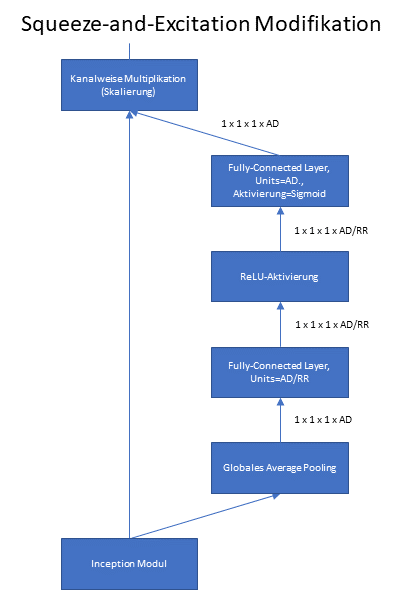
\includegraphics[scale=0.75]{pictures/Inception/SqueezeAndExcitation}
\label{fig:sae}
\end{figure}
